\documentclass{cmn}
\usepackage{ts-arrow}
\usetikzlibrary{shapes.geometric}

\tikzset{
  el/.style={
    draw,
    ellipse,
    inner xsep=-3.75pt,
    inner ysep=3.75pt,
  },
  rect/.style={
    draw,
    rectangle,
    inner xsep=2.5pt,
    inner ysep=5pt,
  },
  level 1/.style={
    level distance=12mm,
    sibling distance=46mm,
  },
  level 2/.style={
    level distance=16mm,
    sibling distance=23mm,
  },
  level 3/.style={
    level distance=16mm,
    sibling distance=22mm,
  },
}

\begin{document}
  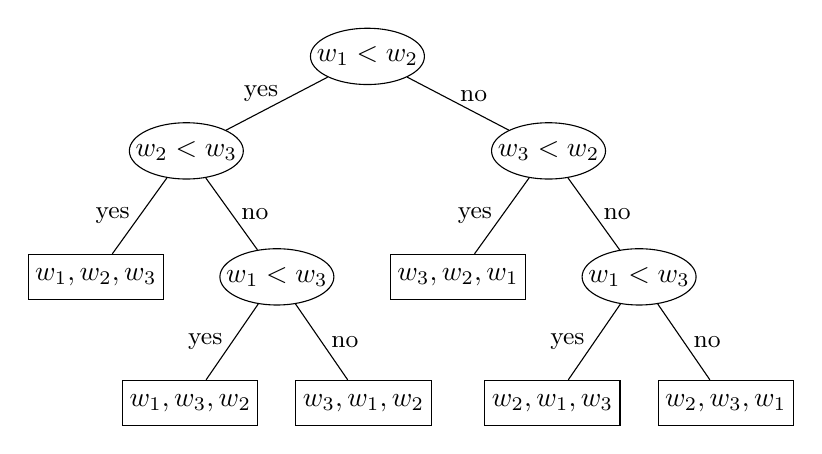
\begin{tikzpicture}
    \node[el] {$w_1 < w_2$}
      child {
        node[el] {$w_2 < w_3$}
        child {
          node[rect] {$w_1,w_2,w_3$}
          edge from parent node[left] {\small yes}
        }
        child {
          node[el] {$w_1 < w_3$}
          child {
            node[rect] {$w_1,w_3,w_2$}
            edge from parent node[left] {\small yes}
          }
          child {
            node[rect] {$w_3,w_1,w_2$}
            edge from parent node[right] {\small no}
          }
          edge from parent node[right] {\small no}
        }
        edge from parent node[left=2mm,above=-1mm] {\small yes}
      }
      child {
        node[el] {$w_3 < w_2$}
        child {
          node[rect] {$w_3,w_2,w_1$}
            edge from parent node[left] {\small yes}
        }
        child {
          node[el] {$w_1 < w_3$}
          child {
            node[rect] {$w_2,w_1,w_3$}
            edge from parent node[left] {\small yes}
          }
          child {
            node[rect] {$w_2,w_3,w_1$}
            edge from parent node[right] {\small no}
          }
          edge from parent node[right] {\small no}
        }
        edge from parent node[right=2mm,above=-1mm] {\small no}
      };
  \end{tikzpicture}
\end{document}
